\textbf{4-1} 试证明自然光通过偏振片后的强度为入射光强的一半，忽略由于吸收、反射和散射等原因引起的光能损失。
\vfill

\textbf{4-2}以横振动的角分布为任意的部分偏振光入射到偏振片，以光线为轴旋转偏振片.

1.试证明, 偏振片旋转一周内, 透射光只有两个光强极大方位和两个光强极小方位, 且极大方位与极小方位垂直.

2. 试证明, 就透过偏振片的透射光而言, 入射的任意部分偏振光等效于适当强度的自然光和线偏振光的组合.

\vfill\newpage
\textbf{4-3} 偏振分束器可把入射的自然光分成两束传播方向互相垂直的线偏振光，其结构如光图4-3-1所示。两个直角玻璃棱镜斜面对斜面合在一起，两斜面之间夹一多层膜，多层膜由高折射率和低折射率材料交替地组合而成。设高折射率为 $n_{H}$ ，低折射率为 $n_{L}$ ，自然光以 $45^{\circ}$ 的入射角入射到多层膜上。

1. 为使反射光为线偏振光, 玻璃棱镜的折射率 $n$ 必须取特殊值, 试导出 $n$ 的公式 .

2. 试问, 为使透射光有最大的偏振度, 高折射率层的厚度 $t_{\mathrm{H}}$ 和低折射率层的厚度 $t_{\mathrm{L}}$ 应怎样决定? 试导出最小厚度的公式 .3. 对于氩离子激光, $\lambda = 514.5 \mathrm{~nm}$ , 以硫化锌为高折射率层, 其折射率 $n_{\mathrm{H}} = 2.38$ , 以冰晶石为低折射率层, 其折射率 $n_{\mathrm{L}} = 1.25$ . 试求 $n$ 和 $t_{\mathrm{H}}, t_{\mathrm{L}}$ 的最小值.

\begin{center}
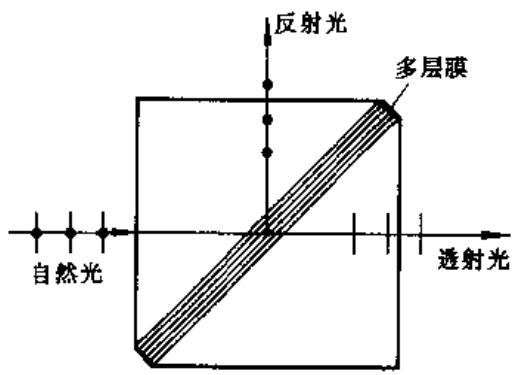
\includegraphics[width=0.3\textwidth]{figures/光图4-3-1.jpg}
\end{center}

\vfill

\textbf{4-4} 介质1和介质2的折射率分别为 $n_1$ 和 $n_2$ ，一线偏振光从介质1向两介质的界面入射，振动方向与入射面的夹角 $\alpha$ 称为振动方位角．试求反射光和折射光的振动方位角．

\vfill\newpage
\textbf{4-5} 一束自然光从空气入射到空气-玻璃界面，入射角 $\theta_{1} = 30^{\circ}$ ，玻璃折射率 $n = 1.50$ 。试求反射光的偏振度。

\vfill

\textbf{4-6} 自然光从空气到玻璃 $(n=1.50)$ 以布儒斯特角入射。

1.试分别计算垂直分量(S分量)和平行分量(P分量)的振幅反射率r，光强反射率R和能流反射率 $\overline{R}$ ；以及振幅透射率t，光强透射率T和能流透射率 $\overline{T}$ 。

2.试求折射光的偏振度。

\vfill\newpage
\textbf{4-7} 玻片堆玻璃板的折射率 $n = 1.54$ ，放置在空气中，自然光以布儒斯特角入射。

1.试求通过第一、二、四块玻璃板后的偏振度。

2.为了使得从玻片堆射出的偏振光达到 $99\%$ 的偏振度，试问至少需要多少块玻璃板？不考虑由吸收和散射等原因引起的光能损失，也不考虑多次反射。

\vfill

\textbf{4-8} 线偏振光向电介质的界面入射。试证明，在全反射条件下，反射光一般为椭圆偏振光。

\vfill\newpage
\textbf{4-9} 界面两侧的折射率分别为 $n_1$ 和 $n_2$ . 光从折射率为 $n_1$ 的第一介质以入射角 $\theta_1$ 入射, 经界面反射. 定义 $S$ 分量和 $P$ 分量的振幅反射率之比为
$$ G = \frac {r _ {P}}{r _ {S}} $$
试证明,第二介质的折射率为
$$ n _ {2} = n _ {1} \sin \theta_ {1} \left[ 1 + \left(\frac {1 - G}{1 + G}\right) ^ {2} \tan \theta_ {1} \right] ^ {\frac {1}{2}} $$
\vfill

\textbf{4-10} 如光图4-10-1所示，一石英晶体棱镜的顶角为 $60^{\circ}$ ，光轴与棱镜主截面垂直。钠黄光在最小偏向角条件下入射，用一焦距为 $1.00\mathrm{m}$ 的透镜聚焦。试求o光和e光两谱线的间距。已知 $n_{\mathrm{o}} = 1.544, n_{\mathrm{e}} = 1.553$ 。

\begin{center}
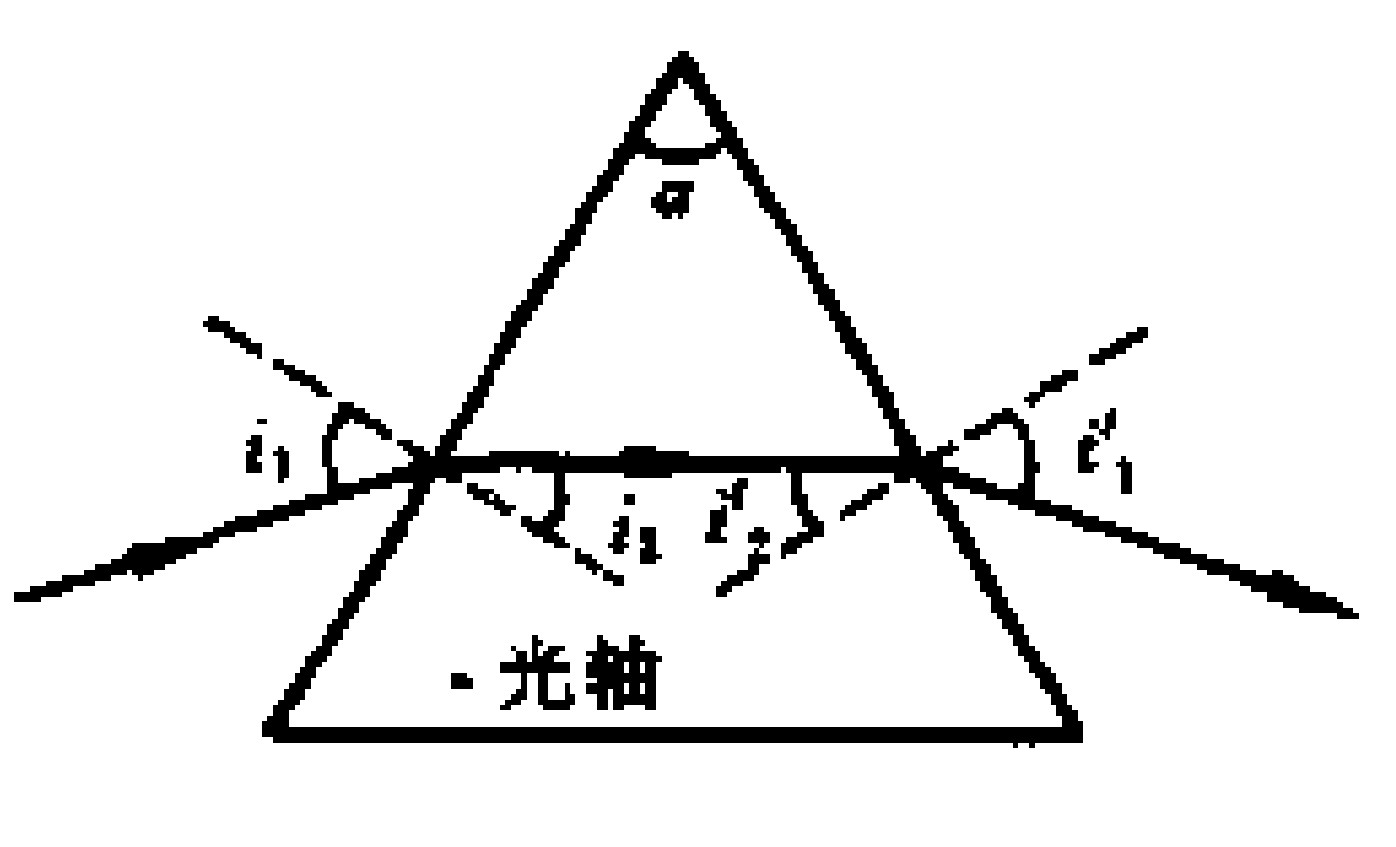
\includegraphics[width=0.3\textwidth]{figures/光图4-10-1.jpg}
\end{center}
\vfill\newpage
\textbf{4-11} 试问用两个透光轴未知的偏振片及一个快轴方向已知的 $\frac{1}{4}$ 波片，怎样确定另一个 $\frac{1}{4}$ 波片的快轴和慢轴。

\vfill

\textbf{4-12} 已知入射光为单色右旋圆偏振光。试利用一透光轴已知的偏振片确定由方解石制成的 $\frac{1}{4}$ 波片的光轴方向。

\vfill\newpage
\textbf{4-13} 通过尼科耳棱镜观察部分偏振光。当尼科耳棱镜从光强为极大的位置转过 $60^{\circ}$ 角时，光强减为一半。试求入射的单色部分偏振光的偏振度。

\vfill

\textbf{4-14} 一强度为 $I_0$ 的右旋圆偏振光垂直通过 $\frac{1}{4}$ 波片，然后通过一尼科耳棱镜. 尼科耳棱镜的主截面 $N$ 在 $\frac{1}{4}$ 波片的快轴方向右旋 $15^{\circ}$ 处。试求最后射出的光的强度。

\vfill\newpage
\textbf{4-15} 偏振片和 $\frac{1}{4}$ 波片可组成一个圆偏振器。自然光通过偏振片后成为线偏振光，若其振动方向与 $\frac{1}{4}$ 波片的光轴方向夹 $45^{\circ}$ 角，则从 $\frac{1}{4}$ 波片射出的是圆偏振光。今有两组同样的圆偏振器，偏振片分别用 $N_{1}$ 和 $N_{2}$ 表示， $\frac{1}{4}$ 波片用 $P_{1}$ 和 $P_{2}$ 表示。两组圆偏振器的相对取向夹一任意角 $\theta$ 并按以下两种方式排列：1. $P_{1}, N_{1}, N_{2}, P_{2}; 2. N_{1}, P_{1}, P_{2}, N_{2}$ ，以自然光入射，光强为 $I_{0}$ ，试求在上述两种情况下，透射光的光强。

\vfill

\textbf{4-16} 如光图4-16-1所示，在平面反射镜上相继地放置一个 $\frac{1}{4}$ 波片和一个偏振片，偏振片的透光轴与 $\frac{1}{4}$ 波片的光轴夹角为 $\theta$ 。光强为 $I_0$ 的自然光垂直入射。试求反射光经上述偏振系统后的光强。


\begin{center}
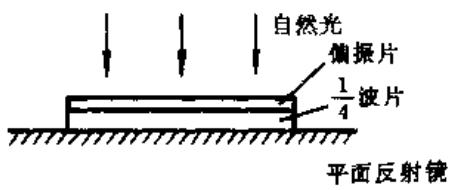
\includegraphics[width=0.3\textwidth]{figures/光图4-16-1.jpg}
\end{center}

\vfill\newpage
\textbf{4-17} 用一偏振片检验椭圆偏振光时，透过偏振片的光强将随偏振片的旋转角度变化。对于已设定的坐标系统，已知合成为椭圆偏振光的两个垂直振动之间的相位差为 $\delta$ 。

1. 试导出透射光强随偏振片旋转角度变化的普遍公式.

2. 试确定椭圆偏振光长、短轴的方位以及相应的透射光强的极大值和极小值.

\vfill

\textbf{4-18} 如光图4-18-1和光图4-18-2所示，入射的椭圆偏振光的强度为 $I_0$ ，椭圆的长短轴之比为2:1，相继地通过晶片C和偏振片N.晶片由负晶体制成，其光轴平行于表面，并与椭圆的短轴一致，o光和e光通过晶片后产生 $\frac{\pi}{3}$ 的相位差，以晶片的光轴为 $x$ 轴，偏振片透光轴N与x 轴的夹角为 $30^{\circ}$ .

1. 若入射光为右旋椭圆偏振光, 试求出射光强 I. 当转动偏振片时, 试问透过的最大和最小光强各为多少? 各在什么方位? 

2. 若入射光为左旋椭圆偏振光, 试问结果如何?


\begin{center}
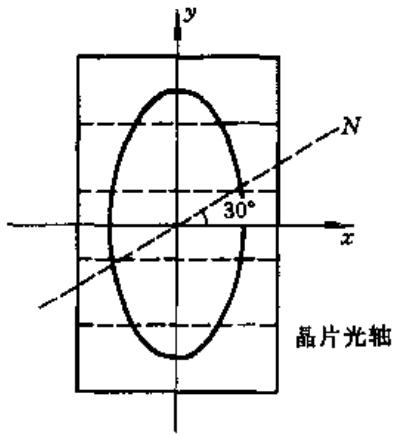
\includegraphics[width=0.3\textwidth]{figures/光图4-18-1.jpg}
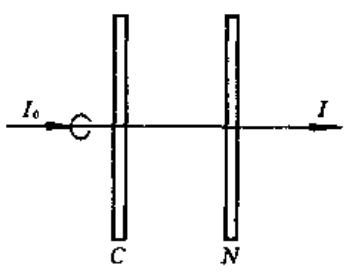
\includegraphics[width=0.3\textwidth]{figures/光图4-18-2.jpg}
\end{center}

\vfill\newpage
\textbf{4-19} 单色部分椭圆偏振光沿 $z$ 方向传播，借助于一偏振片作检验。当偏振片的透光轴与 $x$ 方向一致时，透射强度最大，其值为 $1.5I_0$ ；当透光轴与 $y$ 方向一致时，透射强度最小，其值为 $I_0$ 。

1. 试求透光轴与 $x$ 轴夹任意角 $\theta$ 时的透射强度。

2. 令入射光束先通过一个 $\frac{1}{4}$ 波片，该 $\frac{1}{4}$ 波片的光轴与 $x$ 轴或 $y$ 轴一致。发现当偏振片的透光轴与 $x$ 轴夹 $30^{\circ}$ 角时，透射的强度最大。试求此最大强度，并求入射光中非偏振成分的比例。

\vfill

\textbf{4-20} 线偏振光垂直入射到光轴平行于表面的晶片上，其振动方向与晶片光轴方向之间的夹角为 $\theta$ 。设o光和e光通过晶片后产生的相位差为 $\delta$ ，则从晶片射出的光一般为椭圆偏振光。

1. 试导出决定该椭圆偏振光椭圆长轴方位的公式.2. 试导出椭圆长短轴之比的公式.

\vfill\newpage
\textbf{4-21} 如光图4-21-1所示，在杨氏干涉实验装置中，以单色自然光照射小孔S，幕上将出现场氏干涉条纹，在中央附近干涉极大的强度相对均匀，在较大范围内则将表现出单缝衍射的影响。

1. 若在 S 后放置一偏振片 P, 试问幕上的干涉条纹是否变化? 

2. 若在双孔 $S_{1}$ 和 $S_{2}$ 后再各加一偏振片 $P_{1}$ 和 $P_{2}$ , 且使 $P_{1}$ 和 $P_{2}$ 的透光轴与 P 的透光轴各夹 $45^{\circ}$ 角. 试问幕上的光强分布如何? 

3. 除上述 $P, P_{1}, P_{2}$ 外, 若在屏幕前再放置偏振片 $P_{3}$ , 其透光轴与 P 的透光轴平行, 试问幕上的光强分布如何? 

4. 在第 3 问中, 若 $P_{3}$ 与 P 的透光轴相互垂直, 试问幕上的条纹分布有何变化? 

5. 在第 3 问中, 若去掉偏振片 P, 试问幕上的光强分布如何?


\begin{center}
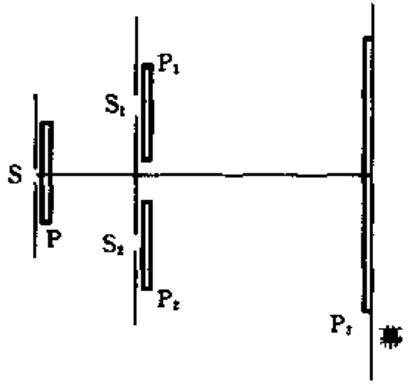
\includegraphics[width=0.3\textwidth]{figures/光图4-21-1.jpg}
\end{center}

\vfill
\newpage
\textbf{4-22} 如光图4-22-1所示，在杨氏干涉装置中双孔 $\mathbf{S}_1$ 和 $\mathbf{S}_2$ 后各放置一个由同样材料制成的厚度均为 $d$ 的晶片 $\mathbf{C}_1$ 和 $\mathbf{C}_2$ ，两晶片的光轴均与表面平行，两光轴相互垂直．试问幕上将观察到什么结果？


\begin{center}
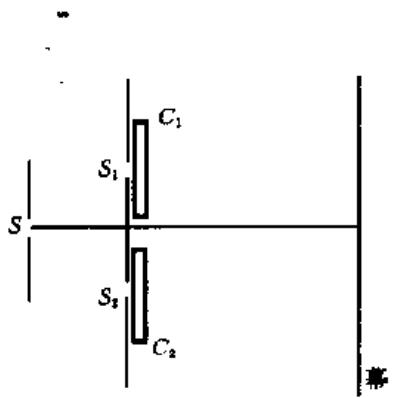
\includegraphics[width=0.3\textwidth]{figures/光图4-22-1.jpg}
\end{center}

\vfill
\textbf{4-23} 两晶片由同种材料制成，第一晶片的快慢轴平行于晶片表面，厚度为 $d$ ，第二晶片为 $\frac{1}{4}$ 波片。两晶片的快轴夹 $45^{\circ}$ 角。波长为 $\lambda$ 的单色线偏振光垂直入射到第一晶片上，相继地通过两个晶片，入射线偏振光的振动方向与 $\frac{1}{4}$ 波片的快轴方向一致。试求从第二晶片透出的光的偏振状态。

\vfill
\newpage
\textbf{4-24} 一厚度 $d = 0.025\mathrm{mm}$ 的方解石晶片，光轴与表面平行，放置在两正交偏振片之间，第一偏振片的透光轴方向与晶片的主截面成 $45^{\circ}$ 角。设可见光(波长为 $400 \sim 700\mathrm{nm}$ 的连续谱)垂直入射。

1. 试问透过第二偏振片的光中缺少哪些波长？

2. 若两偏振片的透光轴互相平行，试问透过第二偏振片的光中缺少哪些波长？计算时不考虑色散效应，即 $n_{\mathrm{o}} - n_{\mathrm{e}} = 0.172$ 与波长无关。

\vfill
\textbf{4-25} 在偏振光干涉的装置中，两尼科耳棱镜的主截面夹 $60^{\circ}$ 角，两者之间插入一顶角 $\alpha = 30^{\prime}$ 的石英尖劈，其光轴平行于表面，尖劈的主截面与两尼科耳棱镜的主截面都成 $30^{\circ}$ 角。以波长为 $589.3\mathrm{nm}$ 的钠黄光垂直入射。试问:

1. 透射光的光强分布.

2. 干涉条纹的反衬度. 已知石英的折射率 $n_{o}=1.54424, n_{e}=1.55335$ .

\vfill
\newpage
\textbf{4-26} 如光图4-26-1所示，两束同频率的平行光与 $z$ 轴的夹角为 $\theta_{1}$ 和 $\theta_{2}$ ，它们分别为左旋圆偏振光和右旋圆偏振光，光强分别为 $I_{1}$ 和 $I_{2}$ ，同时沿 $yz$ 平面入射到位于 $xy$ 平面的屏幕上。试求屏幕上的干涉强度分布和反衬度。

\begin{center}
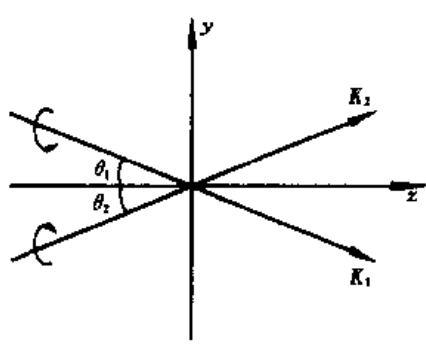
\includegraphics[width=0.25\textwidth]{figures/光图4-26-1.jpg}
\end{center}

\vfill
\textbf{4-27} 如光图4-27-1所示，在杨氏双缝干涉实验装置中，以单色圆偏振光照明狭缝S，在一条狭缝 $\mathbf{S}_1$ 后放置一方解石晶片，晶片的光轴平行于图面和晶片表面，晶片的主折射率为 $n_{\mathrm{o}}$ 和 $n_{\mathrm{e}}$ 。试求幕上干涉条纹的反衬度为最大和最小时晶片的厚度 $t$ 。
\begin{center}
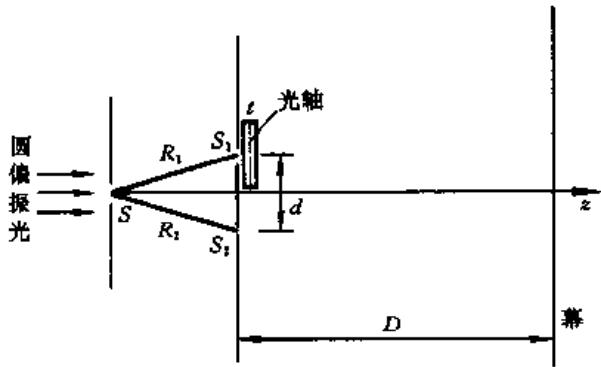
\includegraphics[width=0.35\textwidth]{figures/光图4-27-1.jpg}
\end{center}

\vfill
\newpage
\textbf{4-28} 波长 $\lambda = 500\mathrm{nm}$ 的线偏振光沿 $z$ 方向传播，其电矢量振动方向与 $x$ 轴夹 $45^{\circ}$ 角，通过一克尔盒，盒长 $l = 1.0\mathrm{cm}$ ，盒内介质在 $x$ 方向的电场作用下变为各向异性，主折射率之差为
$$ n _ {x} - n _ {y} = K E ^ {2} $$
式中 E 为电场强度，比例系数 $K = 2.5 \times 10^{-6} \, m^{2}/V^{2}$ ， $n_{x}$ 和 $n_{y}$ 分别是振动方向为 x 和 y 时的折射率。

1. 如光图 4-28-1 所示, 在克尔盒后放置一偏振片, 其偏振化方向与入射光的振动方向垂直. 试求透过偏振片的光最强时电场强度 $E$ 的最小值.

2. 如光图4-28-2所示，将上述克尔盒放置在杨氏干涉装置的双缝之后，克尔盒的上半部加 $x$ 方向的电场，下半部的电场强度保持为零。连续改变上半部的电场强度，幕上干涉条纹的反衬度将出现周期性的变化。忽略光在克尔盒中的折射偏离。试求反衬度 $\gamma = 0$ 和 $\gamma = 1$ 时的电场强度值。


\begin{center}
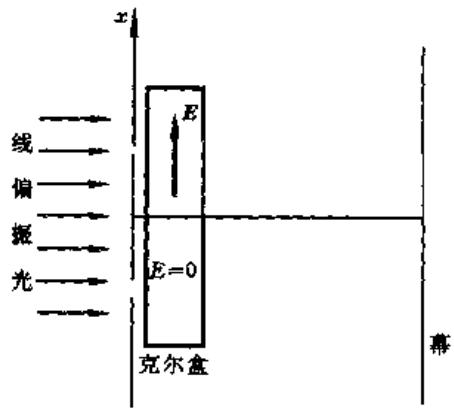
\includegraphics[width=0.3\textwidth]{figures/光图4-28-2.jpg}
\end{center}

\vfill\newpage
\textbf{4-29} 如光图4-29-1所示，石英做成的三棱镜的顶角 $\alpha = 60^{\circ}$ ，光轴与棱镜底边平行。钠黄光的入射角$i_{1}$ 满足最小偏向角条件. 已知石英对钠黄光的折射率 n = 1.544, 对左旋和右旋圆偏振光的折射率之差 $\Delta n = n_{L} - n_{R} = 7.121 \times 10^{-5}$ . 试求从棱镜射出的左旋和右旋圆偏振光之间的夹角 $\Delta \varphi$ .

\begin{center}
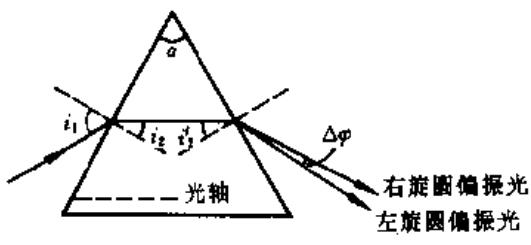
\includegraphics[width=0.3\textwidth]{figures/光图4-29-1.jpg}
\end{center}

\vfill

\textbf{4-30} 如光图4-30-1所示，尼科耳棱镜由方解石晶体做成，在其主截面内， $\angle CAC' = 90^\circ$, $\angle ACC' = 68^\circ$ ，光轴与 $AC$ 之间的夹角为 $48^\circ$ 。正常工作时，自然光沿棱镜的长边方向（即 $S_0M$ 方向）入射，透射光为严格的线偏振光。入射光方向相对 $S_0M$ 方向的任何偏离，例如沿 $S_1M$ 或 $S_2M$ 方向入射，都可能使尼科耳棱镜失去起偏振的作用。试分别计算允许的偏离角 $\theta_1$ 和 $\theta_2$ 。已知方解石的主折射率为 $n_o = 1.658, n_e = 1.486$ ，用于胶合的加拿大胶的折射率 $n = 1.550$ 。

\begin{center}
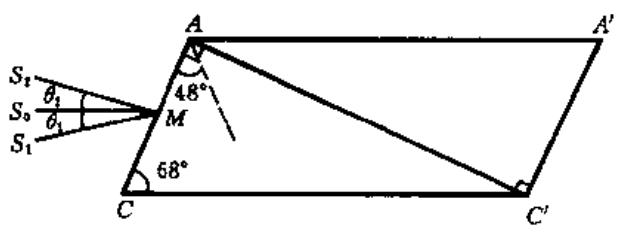
\includegraphics[width=0.3\textwidth]{figures/光图4-30-1.jpg}
\end{center}

\vfill\newpage
\textbf{4-31} 在各向异性晶体中，波法线方向与光线方向一般并不一致。试求冰洲石(方解石)晶体中两者之间的最大夹角，并与石英晶体的对应量作比较。已知冰洲石的主折率为 $n_{\mathrm{o}} = 1.658$ ， $n_{\mathrm{e}} = 1.486$ ；石英的主折射率为 $n_{\mathrm{o}} = 1.544, n_{\mathrm{e}} = 1.553$ 。

\vfill

\textbf{4-32} 折射率为 $n_1$ 的各向同性介质与主折射率为 $n_0$ 和 $n_e$ 的单轴晶体构成一界面。线偏振光从各向同性介质沿晶体的主截面入射到界面上，其振动方向与入射面平行。为使入射光在界面上产生全反射。试问 $n_1$ 必须满足什么条件？全反射的临界角为多大？设晶体光轴与界面法线夹角为 $\varphi$ 。

\vfill\newpage
\textbf{4-33} 单轴晶体中的e光光线在晶体内表面反射时一般不遵从通常的反射定律. 已知晶体的光轴方向与晶体表面的法线之间的夹角为 $\varphi, e$ 光沿主截面入射到内表面上. 试导出e光光线反射时入射角与反射角之间的关系.

\vfill\newpage

\textbf{4-34} 折射率为 $n_1$ 的各向同性介质(介质1)与主折射率为 $n_0$ 和 $n_e$ 的单轴晶体(介质2)构成一界面，晶体光轴与界面法线之间的夹角为 $\varphi$ 。线偏振光从介质1沿晶体主截面斜入射，入射角为 $\theta_i$ ，线偏振光的振动方向与主截面平行。试导出决定振幅反射系数和透射系数的公式。

\vfill\newpage
\textbf{4-35} 试由上题(本章题34)情形验证光的可逆性原理,并由光的可逆性原理推出反射系数和透射系数遵从的斯托克斯倒逆关系.

\vfill

